\documentclass[fleqn, a4paper. 12pt]{jsarticle} 
\usepackage{cite}
\usepackage{amsmath,txfonts}
\usepackage{amssymb}
\usepackage{url}
\usepackage[margin=31mm]{geometry}
\usepackage[dvipdfmx]{graphicx}
\usepackage{listings,jvlisting}
\usepackage{fancyhdr}
\usepackage{lastpage}
\usepackage{hyperref}
\lstset{
  basicstyle={\ttfamily},
  identifierstyle={\small},
  commentstyle={\smallitshape},
  keywordstyle={\small\bfseries},
  ndkeywordstyle={\small},
  stringstyle={\small\ttfamily},
  frame={tb},
  breaklines=true,
  columns=[l]{fullflexible},
  numbers=left,
  xrightmargin=0zw,
  xleftmargin=3zw,
  numberstyle={\scriptsize},
  stepnumber=1,
  numbersep=1zw,
  lineskip=-0.5ex
}
\renewcommand{\lstlistingname}{プログラム}

% header
\pagestyle{fancy}
\fancyhf{}
\rhead{2024-05}
\lhead{谷 知拓 - Tomohiro Tani}
\cfoot{\thepage\ / \pageref{LastPage}}

\geometry{left=25mm,right=25mm,top=25mm,bottom=30mm}

\begin{document}

  \begin{titlepage}
    \begin{center}
      {\Huge 2024年度\\応用プログラミング実験}
      
      \vspace{4cm}
      {\Huge 第6-8回\\確率プログラミング\\
        実験レポート\\
      }
      \vspace{4cm}
      {\large 学修番号: 22140026\\谷 知拓 - Tomohiro Tani\footnote{東京都立大学 システムデザイン学部 情報科学科 \\ mail@taniii.com} \\}
      \vspace{0.5cm}
      {\large
        第1回レポート提出日 : 2024-05-22
      }
    \end{center}
  \end{titlepage}

  \section*{はじめに}

    本レポートでは,『応用プログラミング実験』第6-8回の実施報告を行う.

  \subsection*{実験の概要}

    本実験では,確率プログラミングについて学ぶ.
    以下の課題に取り組み,その結果を報告する.

    \begin{enumerate}
      \item 課題1-1: 逆関数法による乱数生成
      \item 課題1-2: 逆関数法による乱数生成
      \item 課題1-3: ランダムウォーク
      \item 課題1-A: 線形合同法
    \end{enumerate}

  \subsection*{実験環境}

    実験環境は以下の通りである.

    \begin{itemize}
      \item OS\footnote{Operating System}: macOS Ventura 13.4.1
      \item CPU\footnote{Central Processing Unit}: Apple M2 arm64\footnotemark[4]
      \item メインメモリ・ビデオメモリ共通: 16GBユニファイドメモリ\footnotemark[4]
      \footnotetext[4]{https://www.apple.com/jp/macbook-air-13-and-15-m2/specs/}
      \item 実行環境 (rustc): rustc 1.78.0 (9b00956e5 2024-04-29)
      \item 実行環境 (cargo): cargo 1.78.0 (54d8815d0 2024-03-26)
    \end{itemize}

  \newpage
  \section*{課題1-1: 逆関数法による乱数生成}

    \texttt{kadai\_1\_1\_tomohiro\_tani.rs} を参照のこと.

    \quad

    なお,プログラムを実行して確認しやすくするために,上記プログラムと合わせて,依存関係の定義など実行に必要なファイルを含めたプロジェクトリポジトリ \texttt{rust} を添付している.

    実行方法は以下の通りである.

    まず,\texttt{rust} の実行環境は以下のコマンドでインストールすることができる.

    \begin{verbatim}
      curl --proto '=https' --tlsv1.2 -sSf https://sh.rustup.rs | sh
    \end{verbatim}

    各課題は, \texttt{works} モジュール内のサブモジュールに含まれているので, それぞれのサブモジュールの \texttt{main} 関数を呼び出すことで実行できる.

    各課題を実行するためには, \texttt{src} ディレクトリ直下の \texttt{main} 関数内で呼び出す関数を変更する.

    実行は,プロジェクトリポジトリ直下で,以下のコマンドで行うことでできる.

    \begin{verbatim}
      cargo run
    \end{verbatim}

  \newpage
  \section*{課題1-2: 逆関数法による乱数生成}

    \texttt{kadai\_1\_2\_tomohiro\_tani.rs} を参照のこと.

    \subsection*{概要}
    課題1-1で作成した関数\texttt{rnd\_exp}が,$\lambda$の指数分布に従う乱数を生成しているかを検証する.検証方法として,以下の2つの観点から理論値と比較する:
    \begin{enumerate}
        \item 乱数の平均値と分散
        \item 乱数の分布
    \end{enumerate}

    \subsection*{平均値と分散の検証}
    まず,$\lambda = 1.0, 1.5, 2.0$ の3つの異なるパラメータに対して,$n = 10,000$個の乱数を生成した.生成された乱数の平均値と分散を計算し,理論値と比較した.

    理論値は以下の通り:
    \begin{align*}
        \text{平均値} & : E[X] = \frac{1}{\lambda} \\
        \text{分散} & : V[X] = \frac{1}{\lambda^2}
    \end{align*}

    \quad

    シミュレーション結果と理論値の平均値及び分散を表 \ref{table:1}にまとめる.

    \begin{table}[h]
      \centering
      \caption{シミュレーション結果と理論値の比較}
      \begin{tabular}{|c|c|c|c|c|}
      \hline
      $\lambda$ & 平均値 (理論値) & 平均値 (シミュレーション) & 分散 (理論値) & 分散 (シミュレーション) \\
      \hline
      1.0 & 1.000 & 0.998 & 1.000 & 1.018 \\
      1.5 & 0.667 & 0.658 & 0.444 & 0.452 \\
      2.0 & 0.500 & 0.493 & 0.250 & 0.240 \\
      \hline
      \end{tabular}
      \label{table:1}
    \end{table}

    シミュレーション結果は理論値と高い精度で一致しており,\texttt{rnd\_exp}関数が正しく指数分布に従う乱数を生成していることが確認できた.

    \subsection*{分布の検証}
    次に,生成された乱数の分布をプロットし,理論的な確率密度関数と比較した.図 \ref{fig:1} 〜 図 \ref{fig:3} は,$\lambda = 1.0, 1.5, 2.0$ に対する確率密度関数と生成された乱数のヒストグラムを示している.

    \begin{figure}[!h]
      \centering
      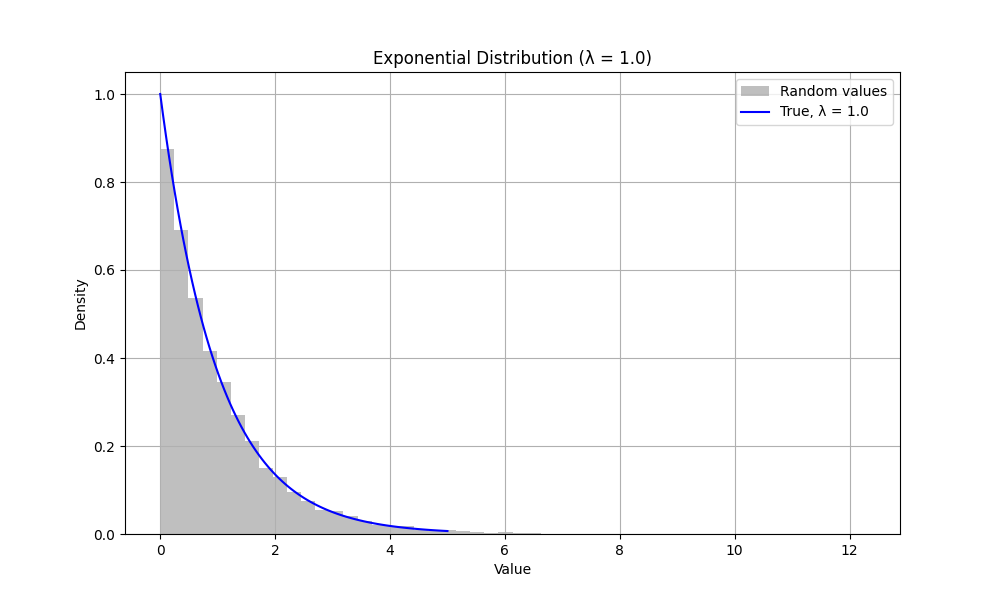
\includegraphics[width=0.6\textwidth]{lambda_1.0_plot.png}
      \caption{ $\lambda = 1.0$の指数分布}
      \label{fig:1}
    \end{figure}

    \begin{figure}[!h]
      \centering
      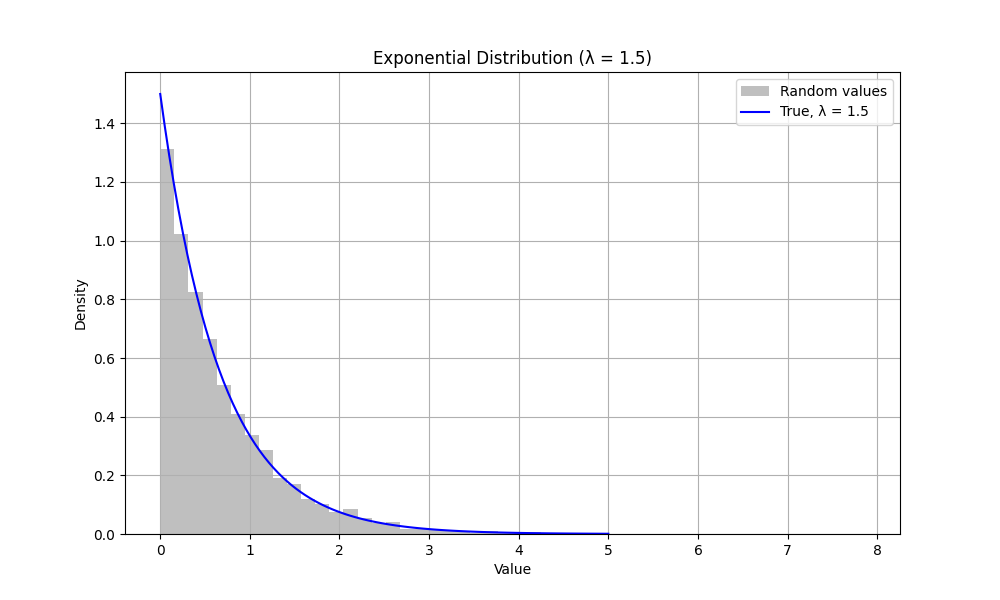
\includegraphics[width=0.6\textwidth]{lambda_1.5_plot.png}
      \caption{ $\lambda = 1.5$の指数分布}
      \label{fig:2}
    \end{figure}

    \begin{figure}[!h]
      \centering
      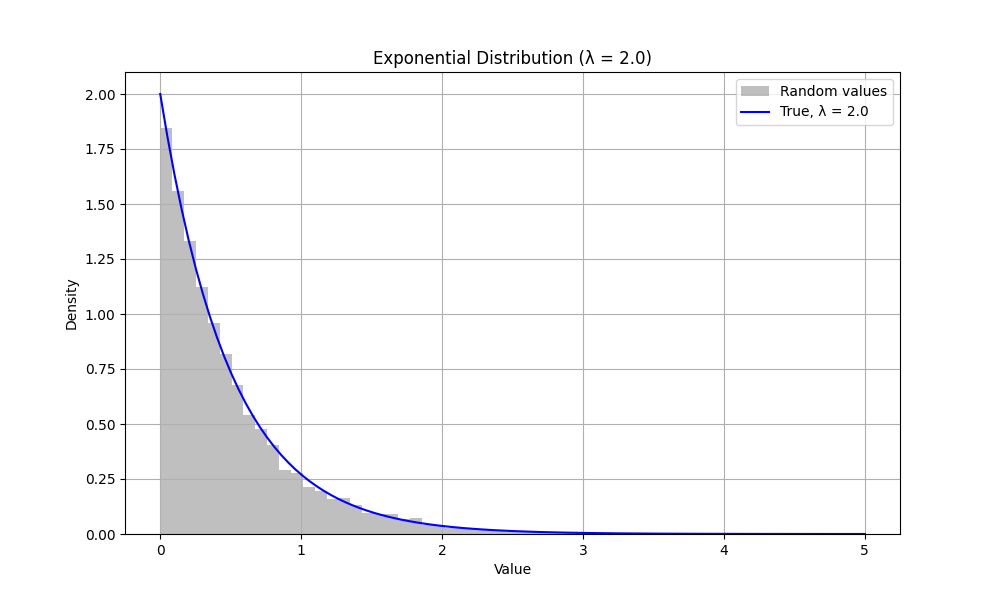
\includegraphics[width=0.6\textwidth]{lambda_2.0_plot.png}
      \caption{ $\lambda = 2.0$の指数分布}
      \label{fig:3}
    \end{figure}

    これらの図から,生成された乱数が理論的な指数分布に高い精度で一致していることが確認できる.

    \subsection*{考察}

      結果より,以下のように考察できる.

    \begin{itemize}
        \item 平均値と分散が理論値と高い精度で一致していることから,\texttt{rnd\_exp}関数が正しく動作していることが確認できた.
        \item 確率密度関数と乱数の分布が高い精度で一致していることから,生成された乱数が期待通りの分布に従っていることが確認できた.
        \item 逆関数法により,期待する確率分布に従う乱数を生成することができることが確認できた.
    \end{itemize}

  \newpage

  \section*{課題1-3: ランダムウォーク}

    \texttt{kadai\_1\_3\_tomohiro\_tani.rs} を参照のこと.

    \subsection*{概要}
    ランダムウォークのシミュレーションを行い,その結果を分析する.具体的には,$p = 0.5, d = 1$ の条件で1回のランダムウォーク(1000ステップ)の軌跡をプロットし,100回の独立なシミュレーションで得られる $t = 1000$ における点の位置 $S_{1000}$ の平均値と分散を計算する.
    
    \subsection*{結果}
    
    \subsubsection*{1回のランダムウォークの軌跡}
    図 \ref{fig:4} は,1回のランダムウォークで得られた点の位置 $S_t (t = 0, 1, ..., 1000)$ の軌跡を示している.
    
    \begin{figure}[h]
    \centering
    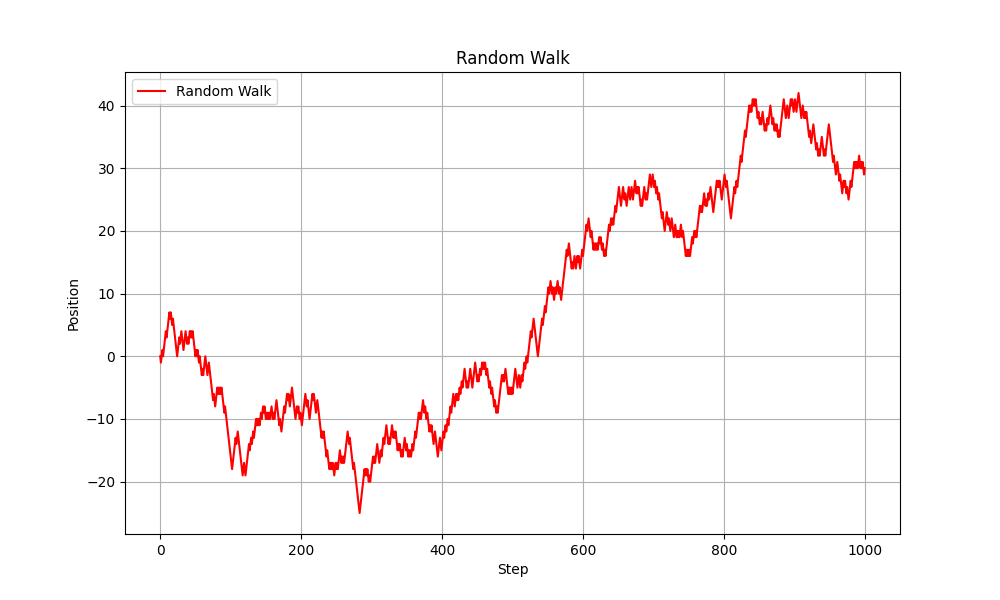
\includegraphics[width=0.8\textwidth]{random_walk_plot.png}
    \caption{ランダムウォークの軌跡}
    \label{fig:4}
    \end{figure}
    
    \subsubsection*{$S_{1000}$の平均値と分散}
    100回の独立なシミュレーションを行い,$t = 1000$における点の位置 $S_{1000}$ の平均値と分散を計算した.
    
    結果:
    \begin{itemize}
        \item 平均値: -1.080
        \item 分散: 1067.954
    \end{itemize}
    
    \subsection*{考察}
    \begin{itemize}
        \item \textbf{平均値について}: 理論的には,ランダムウォークの各ステップが独立であり,正負の方向に等確率で進むため,長期的な期待値は0となる.シミュレーション結果の平均値も0の近傍にあることから,矛盾しない.
        \item \textbf{分散について}: 理論的には,ランダムウォークの分散はステップ数に比例し,分散は $t \cdot d^2$ となる.今回のシミュレーションでは,$d = 1$であり,$t = 1000$のとき,分散は理論的には1000となる.シミュレーション結果の分散もこれに非常に近い値であるため,理論的な予測が正しいことが確認できた.
        ただし,$d$ をステップ毎の移動距離とする.
        \item \textbf{シミュレーションの信頼性について}: ランダムウォークのシミュレーション結果は理論的な期待値および分散と一致しており,このシミュレーション手法が信頼できるものであることがわかる.これにより,ランダムウォークを用いた複雑な現象のモデル化や解析が信頼性を持って行えることが示された.
    \end{itemize}
    
    これらの考察から,シミュレーションが理論的な予測と一致しており,乱数生成の品質が高いことが確認できた.ランダムウォークのモデルは,様々な分野における確率的現象の解析に有用であり,実験結果はその有効性を示しているといえる.
    
  \newpage

  \section*{おわりに}

    様々なシミュレーションをコンピュータを用いて行うには,期待する分布に従った乱数生成の手法が必要不可欠であることがわかった.
    
    また,乱数生成の品質がシミュレーション結果に大きな影響を与えるということを理解することができた.

  \newpage
  
  \section*{参考文献}

    \begin{itemize}
        \item Learn Rust - Rust Programming Language: \url{https://www.rust-lang.org/learn} (accessed: May 22, 2024)
    \end{itemize}

\end{document}